% Created by tikzDevice version 0.12.3.1 on 2021-12-15 14:08:27
% !TEX encoding = UTF-8 Unicode
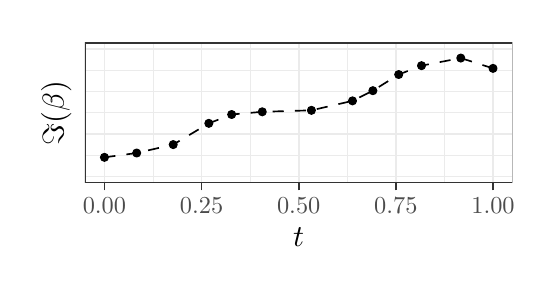
\begin{tikzpicture}[x=1pt,y=1pt]
\definecolor{fillColor}{RGB}{255,255,255}
\path[use as bounding box,fill=fillColor,fill opacity=0.00] (0,0) rectangle (180.67, 86.72);
\begin{scope}
\path[clip] (  0.00,  0.00) rectangle (180.67, 86.72);
\definecolor{drawColor}{RGB}{255,255,255}
\definecolor{fillColor}{RGB}{255,255,255}

\path[draw=drawColor,line width= 0.6pt,line join=round,line cap=round,fill=fillColor] (  0.00,  0.00) rectangle (180.67, 86.72);
\end{scope}
\begin{scope}
\path[clip] ( 20.71, 30.69) rectangle (175.17, 81.22);
\definecolor{fillColor}{RGB}{255,255,255}

\path[fill=fillColor] ( 20.71, 30.69) rectangle (175.17, 81.22);
\definecolor{drawColor}{gray}{0.92}

\path[draw=drawColor,line width= 0.3pt,line join=round] ( 20.71, 40.64) --
	(175.17, 40.64);

\path[draw=drawColor,line width= 0.3pt,line join=round] ( 20.71, 55.95) --
	(175.17, 55.95);

\path[draw=drawColor,line width= 0.3pt,line join=round] ( 20.71, 71.27) --
	(175.17, 71.27);

\path[draw=drawColor,line width= 0.3pt,line join=round] ( 45.29, 30.69) --
	( 45.29, 81.22);

\path[draw=drawColor,line width= 0.3pt,line join=round] ( 80.39, 30.69) --
	( 80.39, 81.22);

\path[draw=drawColor,line width= 0.3pt,line join=round] (115.50, 30.69) --
	(115.50, 81.22);

\path[draw=drawColor,line width= 0.3pt,line join=round] (150.60, 30.69) --
	(150.60, 81.22);

\path[draw=drawColor,line width= 0.6pt,line join=round] ( 20.71, 32.98) --
	(175.17, 32.98);

\path[draw=drawColor,line width= 0.6pt,line join=round] ( 20.71, 48.30) --
	(175.17, 48.30);

\path[draw=drawColor,line width= 0.6pt,line join=round] ( 20.71, 63.61) --
	(175.17, 63.61);

\path[draw=drawColor,line width= 0.6pt,line join=round] ( 20.71, 78.93) --
	(175.17, 78.93);

\path[draw=drawColor,line width= 0.6pt,line join=round] ( 27.74, 30.69) --
	( 27.74, 81.22);

\path[draw=drawColor,line width= 0.6pt,line join=round] ( 62.84, 30.69) --
	( 62.84, 81.22);

\path[draw=drawColor,line width= 0.6pt,line join=round] ( 97.94, 30.69) --
	( 97.94, 81.22);

\path[draw=drawColor,line width= 0.6pt,line join=round] (133.05, 30.69) --
	(133.05, 81.22);

\path[draw=drawColor,line width= 0.6pt,line join=round] (168.15, 30.69) --
	(168.15, 81.22);
\definecolor{drawColor}{RGB}{0,0,0}

\path[draw=drawColor,line width= 0.6pt,dash pattern=on 4pt off 4pt ,line join=round] ( 27.74, 39.86) --
	( 39.39, 41.43) --
	( 52.59, 44.47) --
	( 65.46, 52.15) --
	( 73.71, 55.34) --
	( 84.77, 56.32) --
	(102.53, 56.85) --
	(117.37, 60.27) --
	(124.74, 63.95) --
	(134.07, 69.79) --
	(142.31, 72.99) --
	(156.50, 75.74) --
	(168.15, 72.01);
\definecolor{fillColor}{RGB}{0,0,0}

\path[draw=drawColor,line width= 0.4pt,line join=round,line cap=round,fill=fillColor] ( 27.74, 39.86) circle (  1.43);

\path[draw=drawColor,line width= 0.4pt,line join=round,line cap=round,fill=fillColor] ( 39.39, 41.43) circle (  1.43);

\path[draw=drawColor,line width= 0.4pt,line join=round,line cap=round,fill=fillColor] ( 52.59, 44.47) circle (  1.43);

\path[draw=drawColor,line width= 0.4pt,line join=round,line cap=round,fill=fillColor] ( 65.46, 52.15) circle (  1.43);

\path[draw=drawColor,line width= 0.4pt,line join=round,line cap=round,fill=fillColor] ( 73.71, 55.34) circle (  1.43);

\path[draw=drawColor,line width= 0.4pt,line join=round,line cap=round,fill=fillColor] ( 84.77, 56.32) circle (  1.43);

\path[draw=drawColor,line width= 0.4pt,line join=round,line cap=round,fill=fillColor] (102.53, 56.85) circle (  1.43);

\path[draw=drawColor,line width= 0.4pt,line join=round,line cap=round,fill=fillColor] (117.37, 60.27) circle (  1.43);

\path[draw=drawColor,line width= 0.4pt,line join=round,line cap=round,fill=fillColor] (124.74, 63.95) circle (  1.43);

\path[draw=drawColor,line width= 0.4pt,line join=round,line cap=round,fill=fillColor] (134.07, 69.79) circle (  1.43);

\path[draw=drawColor,line width= 0.4pt,line join=round,line cap=round,fill=fillColor] (142.31, 72.99) circle (  1.43);

\path[draw=drawColor,line width= 0.4pt,line join=round,line cap=round,fill=fillColor] (156.50, 75.74) circle (  1.43);

\path[draw=drawColor,line width= 0.4pt,line join=round,line cap=round,fill=fillColor] (168.15, 72.01) circle (  1.43);
\definecolor{drawColor}{gray}{0.20}

\path[draw=drawColor,line width= 0.6pt,line join=round,line cap=round] ( 20.71, 30.69) rectangle (175.17, 81.22);
\end{scope}
\begin{scope}
\path[clip] (  0.00,  0.00) rectangle (180.67, 86.72);
\definecolor{drawColor}{gray}{0.20}

\path[draw=drawColor,line width= 0.6pt,line join=round] ( 27.74, 27.94) --
	( 27.74, 30.69);

\path[draw=drawColor,line width= 0.6pt,line join=round] ( 62.84, 27.94) --
	( 62.84, 30.69);

\path[draw=drawColor,line width= 0.6pt,line join=round] ( 97.94, 27.94) --
	( 97.94, 30.69);

\path[draw=drawColor,line width= 0.6pt,line join=round] (133.05, 27.94) --
	(133.05, 30.69);

\path[draw=drawColor,line width= 0.6pt,line join=round] (168.15, 27.94) --
	(168.15, 30.69);
\end{scope}
\begin{scope}
\path[clip] (  0.00,  0.00) rectangle (180.67, 86.72);
\definecolor{drawColor}{gray}{0.30}

\node[text=drawColor,anchor=base,inner sep=0pt, outer sep=0pt, scale=  0.88] at ( 27.74, 19.68) {0.00};

\node[text=drawColor,anchor=base,inner sep=0pt, outer sep=0pt, scale=  0.88] at ( 62.84, 19.68) {0.25};

\node[text=drawColor,anchor=base,inner sep=0pt, outer sep=0pt, scale=  0.88] at ( 97.94, 19.68) {0.50};

\node[text=drawColor,anchor=base,inner sep=0pt, outer sep=0pt, scale=  0.88] at (133.05, 19.68) {0.75};

\node[text=drawColor,anchor=base,inner sep=0pt, outer sep=0pt, scale=  0.88] at (168.15, 19.68) {1.00};
\end{scope}
\begin{scope}
\path[clip] (  0.00,  0.00) rectangle (180.67, 86.72);
\definecolor{drawColor}{RGB}{0,0,0}

\node[text=drawColor,anchor=base,inner sep=0pt, outer sep=0pt, scale=  1.10] at ( 97.94,  7.64) {$t$};
\end{scope}
\begin{scope}
\path[clip] (  0.00,  0.00) rectangle (180.67, 86.72);
\definecolor{drawColor}{RGB}{0,0,0}

\node[text=drawColor,rotate= 90.00,anchor=base,inner sep=0pt, outer sep=0pt, scale=  1.10] at ( 13.08, 55.95) {$\Im(\beta)$};
\end{scope}
\end{tikzpicture}
